\newpage
\thispagestyle{empty}
\newgeometry{top=1cm, bottom=0.5cm, outer=1.5cm, inner=2.5cm}
\addcontentsline{toc}{section}{Colophon}
\begin{center}
\begin{figure}[h]
\centering
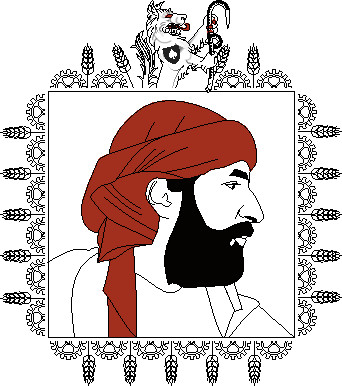
\includegraphics[height=4cm]{portrait.pdf}
\captionsetup{labelformat=empty}
\caption[Effigie de Fauve]{}
\end{figure}

\vspace{3pt}

{\Large À PROPOS DE FAUVE}

\vspace{8pt}

  {\em \color{rouge} ALIAS IDRISS AL IDRISSI}

\vspace{8pt}

{\footnotesize Par Sidi Raiss S. Lridi}

\vspace{10pt}
\end{center}

\shapepar{\authorshape} 
À le présenter autrement que par la façon dont il agirait lui-même, jamais nous ne pourrions nous résoudre. Aussi, lorsqu’on l’interroge, il répond dans un style inhabituellement laconique « Mon existence n’a rien d’extraordinaire », de sa voix grisâtre, comme si les cendres de la guerre de Troie qu’il respirait encore encombraient sa gorge. Sans doute veut-il s’épargner l’embarras auquel le confine pareille question tant les réponses sont multiples. Est-il philosophe ? programmeur ? homme de lettre ? typographe ? archer ? héraldiste ? boxeur ? artiste ? bédéiste ? penseur ? chroniqueur ? Eh bien tout cela à la fois quoiqu’il se refuse d’adopter aucun de ces titres. Or, à choisir parmi ce fatras d’activités une en particulier, c’est laisser entendre d’une part qu’elles sont dissociées les unes des autres, et que pire encore il y’ait une hiérarchie entre elles. Tel est sans doute l’humanisme au sens de la Renaissance, celui qui n’oublie pas les grandes tendances de la polymathie et de l’émancipation, mais qui sait repérer les façons par lesquelles elles se déclinent dans son temps.
Car, sans doute s’agit-il d’un homme autant établi dans le siècle qu’ancré dans l’éternité.

\begin{center}

\includegraphics[height=0.5cm]{engrenage.pdf}
\end{center}

\restoregeometry
